\documentclass{article}
\usepackage[T1]{fontenc}
\usepackage[lithuanian]{babel}
\usepackage{graphicx} % Required for inserting images
\usepackage{float} % For accuratelly placing images
\usepackage[a4paper, margin=2cm]{geometry}
\usepackage[hidelinks]{hyperref}
\usepackage{pdflscape}
\usepackage{longtable}
\usepackage{xltabular}
\usepackage{tabularx}
\usepackage{enumitem}

% For striketrghough
\usepackage{soul}

% For colored highlights 
\usepackage{xcolor}

% BEGIN: FOR SVG
% \usepackage[inkscapelatex=false]{svg}
\usepackage{svg}
\usepackage{amsmath}
% END: FOR SVG

\usepackage{everypage}
\usepackage{lscape} % Ensure landscape pages are recognized
\usepackage{lipsum}

\newcommand{\subsubsubsection}[1]{\paragraph{#1}\mbox{}\\}
\setcounter{secnumdepth}{4}
\setcounter{tocdepth}{3}

\title{
    Įmonės „PTN“ procesų gerinimas\\
    \large vertinamas pagal  "AgilityMod" modelį 
    \large versija 2.0 \\
    \large Komanda „PTN“}
\author{
    Greta Virpšaitė \\
    Rugilė Vasaitytė \\
    Domantas Keturakis \\
    Arnas Vaicekauskas \\
    \textbf{Liudas Kasperavičius (Lyderis)} 
}
\date{Spalis 2024}

\begin{document}
% Globals
\newcommand{\WorkProdIdsList}{}
\newcommand{\ProcIdsList}{}

\newcommand{\CheckUniqueWorkProd}[1]{
    \ifinlist{#1}{\WorkProdIdsList} {
    \PackageError{\WorkProdIdsList}{Work product "#1" already exists}{}
    } {
    \ifinlist{#1}{\ProcIdsList} {
        \PackageError{\ProcIdsList}{"#1" exists as a Process}{}
    } {
     \listgadd{\WorkProdIdsList}{#1}
    }
  }
}

\newcommand{\CheckUniqueProc}[1]{
    \ifinlist{#1}{\ProcIdsList} {
    \PackageError{\ProcIdsList}{Work product "#1" already exists}{}
    } {
    \ifinlist{#1}{\WorkProdIdsList} {
        \PackageError{\WorkProdIdsList}{"#1" exists as a Work product}{}
    } {
     \listgadd{\ProcIdsList}{#1}
    }
  }
}

% Work products
\newcommand{\WorkProdList}{}
\newcommand{\defineWorkProduct}[3]{%
  \expandafter\def\csname identifier#1\endcsname{#2}%
  \expandafter\def\csname name#1\endcsname{#3}%
  \CheckUniqueWorkProd{#2}
  \listgadd{\WorkProdList}{#1}
}
\newcommand{\workProdId}[1]{\textit{\csname identifier#1\endcsname}}
\newcommand{\workProdName}[1]{\csname name#1\endcsname}
\newcommand{\workProd}[1]{\workProdId{#1}. \workProdName{#1}}
\newcommand{\prodWork}[1]{\MakeLowercase{\workProdName{#1}} (\workProdId{#1})}

\newcommand{\describeWorkProd}[2]{
    \expandafter\def\csname desc#1\endcsname{#2}
}
\newcommand{\printRow}[1]{
        \workProdId{#1} &
        \workProdName{#1} &
        \csname desc#1\endcsname \\ \hline
}
\newcommand{\workProdDescriptions}{
    \forlistloop{\printRow}{\WorkProdList}
}

% Processes
\newcommand{\defineProcess}[3]{%
  \expandafter\def\csname procId#1\endcsname{#2}%
  \expandafter\def\csname procName#1\endcsname{#3}%
  \CheckUniqueProc{#2}
  \listgadd{\ProcList}{#1}
}
\newcommand{\processId}[1]{\textit{\csname procId#1\endcsname}}
\newcommand{\processName}[1]{\csname procName#1\endcsname}
\newcommand{\process}[1]{\processId{#1}. \processName{#1}}


\maketitle

\newpage
\tableofcontents

\newpage

\section{Pasiruošimas vertinimui}

\subsection{Vertinimo tikslas}

Procesų gerinimas.

\subsection{Vertinimo apimties apibrėžimas}

\subsubsection{Organizacinė apimtis}
Šiame dokumente modeliuojama įmonės "PTN" departamento „Produktų vystymo“ veikla siekiant pagerinti apibrėžtus procesus (žiūrėti \textbf{1.2.3}  dokumento punktą).

\subsubsection{Aukščiausias vertinamas gebėjimo lygis}

Maksimalus vertinimas, kurį gali pasiekti aspektas yra \textbf{trečias}

\subsubsection{Vertinami aspektai}

Visi įmonės apibrėžti procesai (Žiūrėti pirmą įmonės apibrėžtą dokumentą) vertinami pagal "AgilityMod" modelį

%% Galėsiu padaryti (ARNAS)

\subsection{Duomenų surinkimas}

Duomenis yra/bus? renkami iš deperatemnto "PTN" procesų aprašo dokumento (TODO: čia reikia v1.3 failo pavadinimo/link'o??? i.e. "PTN procesų aprašas v1\_3.pdf")

\section{Vertinimas}

\subsection{Aspektų vertinimas}

\href{https://docs.google.com/spreadsheets/d/1unX_xcZLEGHqQOMCuBBXYvVhYjChxpnq/edit?usp=share_link&ouid=113452949406463366361&rtpof=true&sd=true}{procesų\_vertinimas.xlsx}

\subsection{Vertinimo rezultatai}

\subsubsection{Lentelė}

\begin{figure}[H]%[htpb!]
    \centering
    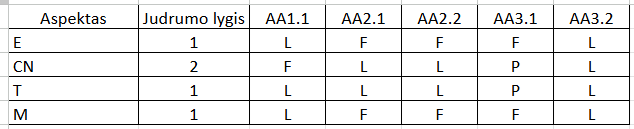
\includegraphics[width=0.85\linewidth]{task-2/images/lentele.png}
\end{figure}

\subsubsection{„Oficialus" gebėjimo profilis}

\begin{figure}[H]%[htpb!]
    \centering
    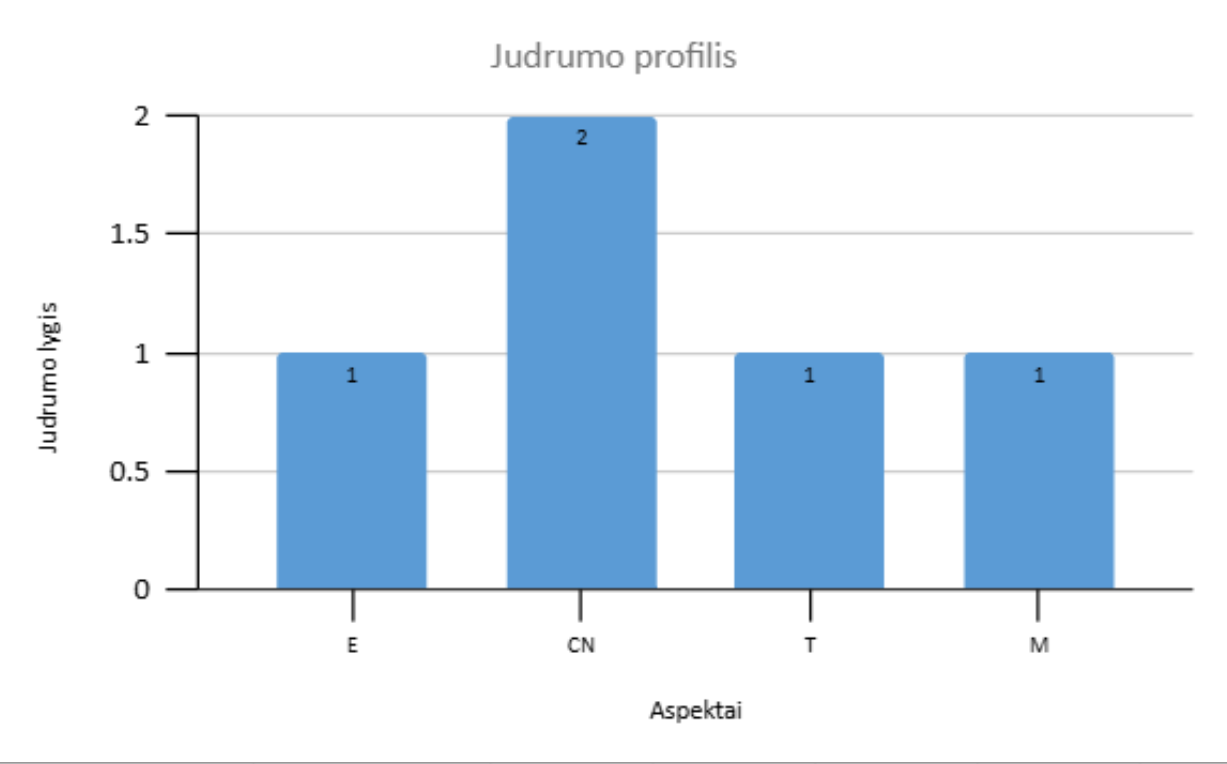
\includegraphics[width=0.85\linewidth]{task-2/images/judrumo-profilis.png}
\end{figure}

\subsubsection{Gebėjimo profilis gerinimui}


\section{Gerinimas}

\subsection{Tikslinis gebėjimo profilis}
\begin{figure}[h]
    \centering
    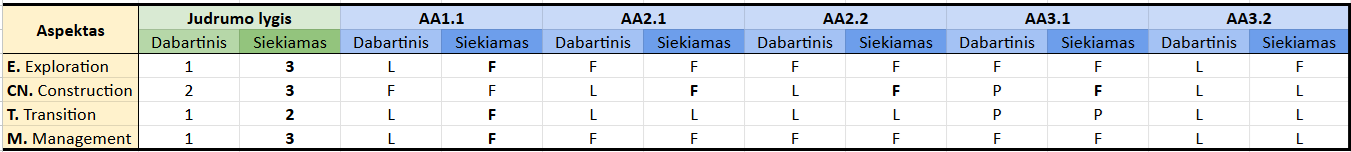
\includegraphics[width=0.75\linewidth]{tikslinis-profilis.png}
    \label{fig:enter-label}
\end{figure}
\subsection{Gerinimo veiksmų planas}

\subsubsection{Exploration aspect}

Šis aspektas pagal esamus procesus yra pasiekęs 1 judrumo lygį. Aspektas gali pasiekti 3 judrumo lygį, jei aspekto atributas
AA 1.1 iš L (77\%) bus pakeltas į F (88\%). Tą pasiekti galima atsižvelgus į šiuo metu procesuose neįgyvendintą E.AP4 aspekto praktiką.

\pagebreak
\subsubsubsection{E.AP4 aspekto praktikos įgyvendinimas}

E.AP4 praktika yra neįgyvendinta N (0\%), ją keliame iki F (100\%) įvykdžius tokius veiklų pakeitimus procesuose:

\subparagraph{Priklausomybių sekimas Projekto užduočių sąrašė (UR)}
\begin{itemize}
    \item \textbf{Vieta:} sekcija 2.3 UR. Užduočių sąrašo rengimas
    \item \textbf{Modifikacija:} pridėti veiklą:
    \begin{quote}
        "Kiekvienai užduočiai (PUS) priskiriamos priklausomybių žymos, nurodant, ar užduotis priklauso nuo kitų užduočių."
    \end{quote}
\end{itemize}

\subparagraph{Sprinto planavimas (SP)}
\begin{itemize}
    \item \textbf{Vieta:} sekcija 2.4.1 SP. Sprinto planavimas (veikla \#2)
    \item \textbf{Modifikacija:} pridėti prie veiklos:
    \begin{quote}
        "Komanda peržiūri užduotis, kurios priklauso nuo kitų užduočių, užduočių sąraše (SUS) ir užtikrina jų tinkamą tvarką"
    \end{quote}
\end{itemize}

\subparagraph{Įgyvendinimo (ĮG) metu keisti priklausomybės statusą}
\begin{itemize}
    \item \textbf{Vieta:} sekcija 2.4.2 ĮG. Įgyvendinimas
    \item \textbf{Modifikacija:} pridėti veiklą:
    \begin{quote}
        "Jeigu rašant programinį kodą, kūrėjui paaiškėja, kad šios užduoties jis negalės atlikti nes pirma turi būti atlikta kita užduotis, kūrėjas sprinto užduočių saraše (\textit{SUS}) pažymi užduotį, nuo kurio priklauso jo atliekama užduotis. Toliau šios užduoties įgyvendinimas nėra tęsiamas iki kol kita užduoties statusas nepasikeičia į DONE."
    \end{quote}
\end{itemize}

\subparagraph{Testavimo (TE) metu keisti priklausomybės statusą}
\begin{itemize}
    \item \textbf{Vieta:} sekcija 2.4.3 TE. Testavimas (veikla \#4)
    \item \textbf{Modifikacija:} pridėti prie veiklos:
    \begin{quote}
        "Jei šio proceso metu nebuvo rasta klaidų užduoties statusas pakeičiamas į DONE ir atnaujinamos užduočių priklausomybių žymos, jeigu yra užduočių, kurios priklauso nuo šios."
    \end{quote}
\end{itemize}

\subparagraph{Kontrolė (KO)}
\begin{itemize}
    \item \textbf{Vieta:} sekcija 2.4.5 KO. Kontrolė (veikla \#1)
    \item \textbf{Modifikacija:} pridėti prie veiklos:
    \begin{quote}
        "Komanda aptaria iškilusius užduočių priklausomybių blokus"
    \end{quote}
\end{itemize}

\subsubsection{Construction aspect}

Aspektas keliamas iš 2 judrumo lygio į 3 judrumo lygį. Tam pasiekti gerinami aspekto atributai:
\begin{enumerate}
\item AA 2.1 iš L (75\%) į F (87,5\%) 
\item AA 2.2 iš L (75\%) į F (87,5\%) 
\item AA 3.1 iš P (25\%) į F (96\%) 
\end{enumerate}

\subsubsubsection{AA 2.1 aspekto atributo iki F gerinimas}

AA 2.1 atributas pagerinamas nuo L (75\%) iki F (87,5\%), pakėlus GP 2.1.2 bendrosios praktikos įvertį nuo 75\% iki 100\%. Tam procesuose atlikti šie pakeitimai

\subparagraph{Kasdieniai Stand-Up susitikimai}
\begin{itemize}
    \item \textbf{Vieta:} Skyrius 2.4 SC. Scrum ciklas
    \item \textbf{Modifikacija:} Nauja veiklą prie \textit{ĮG. Įgyvendinimas}.
    \begin{quote}
   Kiekvieną dieną komanda rengia trumpą Stand-Up susitikimą, kad aptartų progresą, nustatytų kliūtis ir sinchronizuotų veiklas tarp komandos narių. Šis susitikimas paprastai trunka ne ilgiau kaip 15 minučių ir susideda iš trijų pagrindinių punktų: kas buvo padaryta vakar, kas bus daroma šiandien, ir kokios yra šiuo metu esančios kliūtys.
    \end{quote}
\end{itemize}


\subparagraph{Komunikacijos įrankių naudojimą planavimo ir įgyvendinimo etapuose}
\begin{itemize}
    \item \textbf{Vieta:} Skyrius 2.4.1 SP. Sprinto planavimas ir 2.4.2 ĮG. Įgyvendinimas
    \item \textbf{Modifikacija:} Paminėkite Kanban lentų, Slack arba kitų komunikacijos įrankių naudojimą, kurie palaiko Agile principus. 
    \begin{quote}
    Planavimo ir įgyvendinimo metu komanda naudoja komunikacijos įrankius, tokius kaip Kanban lentos ir Slack, kad vizualizuotų darbus, stebėtų progresą ir palaikytų realaus laiko atnaujinimus tarp komandos narių ir suinteresuotųjų šalių. Ši sistema padeda palaikyti užduočių būklės matomumą, leidžiant operatyviai reaguoti į iškilusias problemas.
    \end{quote}
\end{itemize}

\subparagraph{Dokumentuokite komunikaciją Kontrolės (KO) procese}
\begin{itemize}
    \item \textbf{Vieta:} Skyrius 2.4.5 KO. Kontrolė
    \item \textbf{Modifikacija:} Pridėkite žingsnį sprinto retrospektyvos procese, kuriame komandos nariai aptaria naudojamų komunikacijos įrankių ir praktikų efektyvumą.
    \begin{quote}
        Sprinto retrospektyvos metu komandos nariai įvertina komunikacijos praktikų, įskaitant kasdienius Stand-Up susitikimus ir tokių įrankių kaip Kanban lentos ir Slack naudojimo, efektyvumą. Šis grįžtamasis ryšys dokumentuojamas Sprinto Peržiūros Ataskaitoje (SPA), siekiant nuolat gerinti komunikacijos praktikas.
    \end{quote}
\end{itemize}


\subsubsubsection{AA 2.2 Simple aspekto atributo iki F gerinimas}
%-----------------------------------------------MUST FIX START-----------------------------------------------

GP 2.2.2 gerinimas nuo 75\% iki 100\%, siekiant AA 2.2 F (87,5\%) įverčio.

\color{red}Procesuose yra kuriama techninė dokumentacija ir produkto naudojimo instrukcija. Galima suprasti, kad produkto naudojimo instrukcija yra rašoma visada, tuo tarpu techninė dokumentacija turi turėti tam tikrus rašymo kriterijus. Šie išreikštinai procesuose nėra pateikiami, todėl reikia pridėti techninės dokumentacijos rašymo kriterijų sukūrimo veiklą. 

\subsection*{1. Techninės dokumentacijos priemimo kriterijai.}
\textbf{Vieta:} Skyrius 3 Darbo produktų sąrašas \\
\textbf{Papildymas:} Pateikti šablonus su privalomais skyriais skirtingiems dokumentacijos tipams (pvz., techninei, funkcinei dokumentacijai, sprendimų žurnalams).
\begin{quote}
"Projekto darbo produktams pateikiami šablonai, kurie supaprastina dokumentacijos parengimą. Kiekvienam dokumentacijos tipui yra sukurtas šablonas su privalomais skyriais, pvz., techninei dokumentacijai privalomas API aprašymas."
\end{quote}
\color{black}
%-----------------------------------------------MUST FIX END-----------------------------------------------

\subsubsubsection{AA 3.1 aspekto atributo iki F gerinimas}

Norint pasiekti F brandos lygį aspekto atributui AA 3.1, GP 3.1.1 atlikti šie pakeitimai, praktiką pakeliant nuo L (25\%) iki F (100\%):

\subparagraph{Integruoti TDD}
\begin{itemize}
    \item \textbf{Vieta:} Skyrius 2.4.2 ĮG. Įgyvendinimas 
    \item \textbf{Modifikacija:} Pridėti žingsnį, kuris reikalauja kūrėjų naudoti TDD taikomoms užduotims.
    \begin{quote} Programinės įrangos kūrėjai pritaiko testų kūrimo metodą (TDD), prieš pradedant kurti funkcionalumą. TDD užtikrina, kad kiekviena funkcija būtų padengta testais, siekiant išvengti klaidų ir garantuoti kodo kokybę.
    \end{quote}
\end{itemize}

\subparagraph{Pridėti porinio programavimo sesijas}
\begin{itemize}
    \item \textbf{Vieta:} 2.4.2 ĮG. Įgyvendinimas
    \item \textbf{Modifikacija:} Suderinti porinio programavimo sesijas sudėtingoms ar kritinėms užduotims, siekiant užtikrinti kodo kokybę ir dalintis žiniomis.
    \begin{quote} Sudėtingas arba itin svarbias užduotis programuotojai dalinai atlieka naudodami porinio programavimo sesijas. Šių sesijų tikslas yra dalijimasis žiniomis ir momentinė kodo peržiūra.
    \end{quote}
\end{itemize}

Be to, užtikrinamas CI/CD procesas, kuris nenorint kartotis yra aprašytas Transition aspekte, taigi sakykime, kad ši praktika pasiekia F (100\%)

\subsubsection{Transition aspect}

Šis aspektas pagal esamus procesus yra pasiekęs 1 judrumo lygį. Aspektas gali pasiekti 2 judrumo lygi˛ jei aspekto 
atributas AA 1.1 iš L (77\%) bus pakeltas į F.

Toliau gerinkime aspekto atributo praktikas.

\subsubsubsection{T.API1: Sukurkite ir tvarkykite darbo aplinką (angl. Create and Manage the Workspace)}

Išskirti praktikos trūkumai yra tie, jog artefaktai ir trečių šalių bibliotekos turėtų būti saugomos tam skirtose saugyklose, be to kūrimo ir testavimo aplinkos turėtų būti atskirtos, o šių aplinkų valdymas aprašytas išreikštinai. 

\textbf{Reikalingi pakeitimai }
\begin{itemize}
    \item Skyrius „Įgyvendinimas“ (2.4.2 (ĮG)) turi būti papildytas nauja veikla, kurioje aprašomas kodų ir artefaktų tvarkymas:
    \begin{quote}
    „Visi kūrimo, testavimo ir produkcijos aplinkos kodai, trečiųjų šalių bibliotekos ir konfigūracijos turi būti saugomi „GitHub Actions“ arba kitose pasirinktoje versijų valdymo sistemoje.“
    \end{quote}
\end{itemize}

\subsubsubsection{T.API2: Kodo integravimas (angl. Integrate the Code)}

Kodo integravimas turėtų vykti pusiau automatiškai (kodo konfliktų sprendimas negali būti visiškai automatizuotas) ir būti išreikštinai aprašytas, o artefaktų kūrimas turėtų būti automatizuotas

\textbf{Reikalingi pakeitimai}
\begin{itemize}
    \item Skyrius „Testavimas“ (2.4.3 TE) turėtų būti išplėstas su privaloma automatine testavimo strategija, naudojant „GitHub Actions“:
    \begin{quote}
    „Visas kodas turi būti automatiškai tikrinamas prieš integraciją naudojant nuolatinės integracijos ir pristatymo (CI/CD) procesus „GitHub Actions“ platformoje. Automatizuoti testai padeda aptikti konfliktus ir užtikrina kodo kokybę prieš integraciją į pagrindinę šaką.“
    \end{quote}
    \item „Modulinių testų padengimo lygis turi būti ne mažesnis kaip 80\%, o visi pagrindiniai funkcionalumai turi būti patikrinti automatiniais testais.“
\end{itemize}


\subsubsubsection{T.API3: Diegti sprendimą (angl. „Deploy the Solution“) }

\textbf{Reikalingi pakeitimai PDF:}
\begin{itemize}
    \item Skyrius „Įgyvendinimas“ (2.4.2 ĮG) papildyti su informacija apie diegimo proceso automatizavimą:
    \begin{quote}
    „Diegimo procesas turi būti visiškai automatizuotas, naudojant CI/CD diegimo aplinką „GitHub Actions“. Nustatoma, kad kiekviena aplinka turi būti atskirta ir valdyta automatiškai, leidžiant nuosekliai atlikti visus diegimo veiksmus.“
    \end{quote}
    \item „Diegimas į produkcinę aplinką gali vykti tik po to, kai automatizuoti testai patvirtina, kad aplikacija veikia be klaidų.“
\end{itemize}

\textbf{Priežastis:} Automatinis diegimas padeda išvengti žmogaus klaidų diegiant ir leidžia greičiau bei efektyviau atlikti versijų pristatymą.

\subsection*{4. T.API4: Testuoti integruotą sprendimą („Test the Integrated Solution“) }

\textbf{Tikslas:} Užtikrinti, kad integruotas sprendimas būtų ištestuotas funkciniams ir nefunkciniams reikalavimams.

\textbf{Reikalingi pakeitimai PDF:}
\begin{itemize}
    \item Skyrius „Testavimas“ (2.4.3 TE) turėtų būti papildytas su nuoroda į regresinius testus:
    \begin{quote}
    „Visi kodai privalo praeiti regresijos testus prieš pateikiant į aplinką. Regresijos testų rinkinys turi būti sukurtas ir palaikomas taip, kad būtų užtikrintas produkto stabilumas ir kokybė po kiekvieno diegimo.“
    \end{quote}
    \item „Aukštas testų padengimo lygis užtikrina, kad kiekviena funkcija veikia teisingai ir atitinka nustatytus kriterijus.“
\end{itemize}

\textbf{Priežastis:} Regresiniai testai padeda aptikti klaidas, kurios galėjo atsirasti dėl naujų kodo pakeitimų, taip padidinant kodo stabilumą.

\subsection*{5. T.API5: Padaryti progresą matomu („Make the Progress Visible“) }

\textbf{Tikslas:} Užtikrinti, kad visa komanda ir suinteresuotos šalys matytų sprendimo progresą.

\textbf{Reikalingi pakeitimai PDF:}
\begin{itemize}
    \item Skyrius „Kontrolė“ (2.4.5 KO) turėtų būti papildytas su informacija apie darbo eigą:
    \begin{quote}
    „Visa darbo eiga ir progresas turėtų būti stebimi per pasirinktą platformą, pavyzdžiui, „Jira“. Ši platforma leidžia matyti visas užduotis ir jų būseną realiu laiku, įskaitant atliktus pakeitimus ir progresą.“
    \end{quote}
    \item „Kiekviena užduotis turi turėti aiškų aprašymą, nurodant atliktų veiksmų ir būsimų žingsnių seką.“
\end{itemize}

\textbf{Priežastis:} Progreso matomumas padeda komandai stebėti darbo eigą ir laiku aptikti galimas problemas bei nukrypimus nuo plano.

\subsubsection{Management aspect}

Šis aspektas pagal esamus procesus yra pasiekęs 1 judrumo lygi. Aspektas gali pasiekti 2 judrumo lygį, jei
aspekto atributas AA 1.1 iš L bus pakeltas į F.

Pasiekti 2 judrumo lygį galime pakelti M.AP1 ir M.AP3 lygį iki F.

\paragraph{M.AP1 gerinimas siekiant AA 1.1 F lygio}

\subparagraph{pagrįstumo analizė}
\begin{itemize}
    \item \textbf{Vieta:} sekcija 2.1 KĮ. Kliento įtraukimas (veikla \#2).
    \item \textbf{Modifikacija:} pataisyti veiklą ir ją išskirti į dvi:
    \begin{quote}
        "Projektų vadovas, architektas ir analitikas paruošia pradinė projekto viziją tam, kad būtų patvirtintas projekto įgyvendinamumas ir suderinta bendra projekto kryptis su SŠ. Jie taip pat atlieka pagrįstumo analizę, siekdami įvertinti, ar kliento poreikiai (KP) yra įgyvendinami. 
    \end{quote}
    
    \begin{quote}
        "Projektų vadovas, architektas ir analitikas  atsižvelgdami į projekto viziją, pagrįstumo analizę, departamento patirtį su kitais projektais (PAT) bei projekto apimtimi (PA) nustato laiko, kainos ir žmogiškųjų išteklių sąmatą (IS). Laikas, kaina (nustatyti iš IS), projekto apimtis (PA), produkto perdavimo sąlygos ir adaptacinio laikotarpio terminas tuomet yra teisiškai įforminami sutartyje (KS)."
    \end{quote}
\end{itemize}

\paragraph{M.AP8 gerinimas siekiant AA 1.1 F lygio}

\subparagraph{Rizikų įvertinimas}
\begin{itemize}
    \item \textbf{Vieta:} sekcija 2.1 KĮ. Klientų įtraukimas
    \item \textbf{Modifikacija:} pridėti veiklą ir produktas:
    \begin{quote}
        "Analitikas įvertina projekto rizikas (PR)."
    \end{quote}
\end{itemize}
% ČIA NAUJAS WORK PRODUCT

\subparagraph{Rizikų sekimas}
\begin{itemize}
    \item \textbf{Vieta:} sekcija 2.4.5 KO. Kontrolė
    \item \textbf{Modifikacija:} pridėti veiklą:
    \begin{quote}
        "Projekto vadovas peržiūri projekto rizikas (PR) ir dokumentuoja neatitikimus".
    \end{quote}
\end{itemize}

\subparagraph{Rizikų sekimas}
\begin{itemize}
    \item \textbf{Vieta:} sekcija 2.4.5 KO. Kontrolė (veikla \#3)
    \item \textbf{Modifikacija:} pridėti prie veiklos:
    \begin{quote}
        "Remiantis grįžtamojo ryšio registru (GRR) ir laiko valdymo ataskaita, dokumentuotais neatitikimais projekto vadovas atlieka projekto užduočių sąrašo (PUS) atnaujinimą, prireikus, užduočių prioritetų keitimą, pasakojimo vienetu intervalo (PVI) patikslinimą. Šie pakeitimai fiksuojami sprinto peržiuros ataskaitoje (SPA)."
    \end{quote}
\end{itemize}


\end{document}
